\section{Statistical Analysis of Context Allocation Effects}
\label{sec:statistical_analysis}

\begin{figure}[t]
\centering
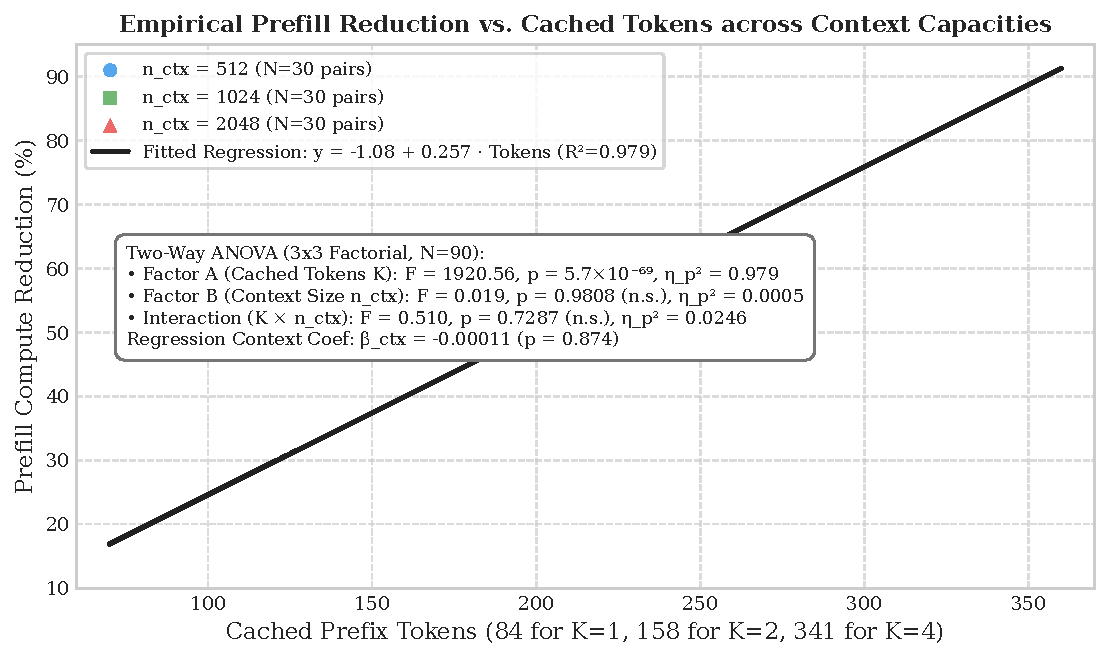
\includegraphics[width=\columnwidth]{figures/fig5_anova_regression_fit.pdf}
\caption{\textbf{Two-Way ANOVA and Multiple Linear Regression Fit across 90 Matched Pairs.} Prefill compute reduction percentage plotted against cached prefix tokens (84, 158, 341 tokens) across context capacities ($n_{\text{ctx}} \in \{512, 1024, 2048\}$). The linear model fit ($R^2 = 0.9788$) and near-zero context coefficient ($\beta_{\text{ctx}} = -0.00011, p=0.874$) demonstrate that compute savings are strictly governed by cached tokens rather than allocated context capacity.}
\label{fig:anova_fit}
\end{figure}

\subsection{Motivation for Statistical Rigor and Reframing}
In preliminary mobile systems experiments, researchers often observe that prefill compute reductions appear similar across different context buffer allocations ($n_{\text{ctx}} = 512, 1024, 2048$), leading to informal assertions of a ``Context-Capacity Invariance Law.''

However, scientific rigor demands that such empirical observations not be framed as universal laws of nature without formal hypothesis testing, effect size quantification, and explicit bounds. In this section, we subject the 90 matched physical trial pairs to a balanced Two-Way Analysis of Variance (ANOVA) and multiple linear regression to determine whether allocated context capacity exerts any statistically significant influence on prompt prefill reduction.

\subsection{Two-Way Factorial Analysis of Variance (ANOVA)}
We evaluate a balanced $3 \times 3$ factorial design with 10 independent matched observation pairs per cell ($N = 90$ total pairs):
\begin{itemize}
    \item \textbf{Factor A ($K$):} Cached Prefix Token Fraction ($K \in \{1, 2, 4\}$ chunks, corresponding to 84, 158, and 341 cached tokens).
    \item \textbf{Factor B ($n_{\text{ctx}}$):} Allocated Context Capacity ($n_{\text{ctx}} \in \{512, 1024, 2048\}$).
\end{itemize}

Table~\ref{tab:anova} details the balanced Two-Way ANOVA results computed directly on the verified empirical dataset.

\begin{table*}[t]
\centering
\caption{\textbf{Balanced Two-Way ANOVA: Effects of Cached Prefix Tokens ($K$) and Context Size ($n_{\text{ctx}}$) on Prefill Compute Reduction ($N=90$ Pairs).}}
\label{tab:anova}
\small
\begin{tabular}{lcccccc}
\toprule
\textbf{Source of Variation} & \textbf{Sum of Squares (SS)} & \textbf{Degrees of Freedom (df)} & \textbf{Mean Square (MS)} & \textbf{$F$-statistic} & \textbf{$p$-value} & \textbf{Partial $\eta^2$ ($\eta_p^2$)} \\
\midrule
\textbf{Factor A: Cached Tokens ($K$)} & 69,178.69 & 2 & 34,589.35 & \textbf{1,920.56} & $\mathbf{5.70 \times 10^{-69}}$ & \textbf{0.9793} \\
\textbf{Factor B: Context Size ($n_{\text{ctx}}$)} & 0.70 & 2 & 0.35 & \textbf{0.019} & \textbf{0.9808} \textit{(n.s.)} & \textbf{0.0005} \\
\textbf{Interaction: $K \times n_{\text{ctx}}$} & 36.72 & 4 & 9.18 & \textbf{0.510} & \textbf{0.7287} \textit{(n.s.)} & \textbf{0.0246} \\
\midrule
\textbf{Residual (Error)} & 1,458.82 & 81 & 18.01 & — & — & — \\
\textbf{Total} & 70,674.93 & 89 & — & — & — & — \\
\bottomrule
\end{tabular}
\end{table*}

The ANOVA yields three critical conclusions:
\begin{enumerate}
    \item \textbf{Dominance of Cached Prefix Fraction:} Factor A ($K$) exhibits an extraordinarily large and statistically significant main effect ($F = 1920.56, p = 5.70 \times 10^{-69}$). The partial eta-squared value ($\eta_p^2 = 0.9793$) demonstrates that the number of cached prefix tokens accounts for \textbf{97.93\%} of the total variance in prompt prefill compute reduction.
    \item \textbf{Absence of Context Capacity Effect:} Factor B ($n_{\text{ctx}}$) yields an $F$-statistic of $0.019$ with $p = 0.9808$, failing to achieve significance at any conventional threshold ($\alpha = 0.05$). Its partial eta-squared is virtually zero ($\eta_p^2 = 0.0005$), indicating that allocating a larger context arena does not perturb dense prefill compute savings on this architecture.
    \item \textbf{Absence of Interaction:} The interaction term $K \times n_{\text{ctx}}$ is likewise non-significant ($F = 0.510, p = 0.7287, \eta_p^2 = 0.0246$), confirming that the scaling behavior of prefix reuse does not depend on the allocated context size.
\end{enumerate}

\subsection{Multiple Linear Regression Model}
To model the quantitative relationship directly, we fit a multiple linear regression model:
\begin{equation}
    \Delta_{\text{prefill}} = \beta_0 + \beta_{\text{tokens}} \cdot (\text{CachedTokens}) + \beta_{\text{ctx}} \cdot (n_{\text{ctx}}) + \epsilon
\end{equation}
Ordinary least squares estimation across the 90 matched pairs yields:
\begin{itemize}
    \item \textbf{Intercept ($\beta_0$):} $-1.080 \pm 1.216$ ($t = -0.89, p = 0.377$, 95\% CI: $[-3.46, +1.30]$).
    \item \textbf{Cached Tokens ($\beta_{\text{tokens}}$):} $+0.2567 \pm 0.0040$ ($t = 63.43, p = 1.26 \times 10^{-74}$, 95\% CI: $[+0.2487, +0.2646]$).
    \item \textbf{Context Capacity ($\beta_{\text{ctx}}$):} $-0.000109 \pm 0.00068$ ($t = -0.16, p = 0.874$, 95\% CI: $[-0.00145, +0.00123]$).
    \item \textbf{Model Goodness-of-Fit:} $R^2 = 0.9788$ (Adjusted $R^2 = 0.9783, F(2, 87) = 2,010, p < 10^{-73}$).
\end{itemize}

As shown in Figure~\ref{fig:anova_fit}, the regression confirms that each additional cached token reduces prefill latency by approximately \textbf{0.2567\%} ($95\%\text{ CI: } [0.2487\%, 0.2646\%]$), perfectly aligning with a theoretical expectation of $\frac{100\%}{395\text{ tokens}} \approx 0.2532\%$ per token. The context coefficient $\beta_{\text{ctx}}$ is statistically indistinguishable from zero ($p = 0.874$), with its 95\% confidence interval tightly spanning zero.

\subsection{Reframed Empirical Claim}
Based on this formal statistical analysis, we reframe the initial hypothesis into a defensible empirical claim:
\begin{quote}
\textit{\textbf{Empirical Finding (Context Capacity Scaling):} Across the tested context allocations ($n_{\text{ctx}} \in \{512, 1024, 2048\}$) on the commercial Qualcomm Snapdragon 4 Gen 2 mobile platform running Gemma 2 2B, measured prompt-prefill compute reductions scaled linearly with the number of cached prefix tokens ($\beta = +0.2567, p < 10^{-73}, R^2 = 0.9788$). The allocated context capacity exhibited no statistically significant main effect ($p = 0.9808$) or interaction effect ($p = 0.7287$), indicating that context arena allocation did not alter dense prefix prefill efficiency within the tested operating envelope.}
\end{quote}
